\documentclass[10pt]{article}
\usepackage{icmlko}

\icmlmeta{IP 파운데이션 월드모델}{500}{「무관 배경」은 배경이 아니라 도메인 이름표였다}{상태 $s$ 를 세 층으로 갈라 한 층씩 붙여 재니, 이득의 전부가 도메인 \emph{사이}에 있었다}

\begin{document}

\twocolumn[
\icmlheader

\begin{abstract}
이 실험실의 상태 $s$ 는 오래 \textbf{채널 하나}였다 --- 학습쌍 1{,}063개 전부에서
$s$ 는 「액션 앞 90일 일별 위키 조회수」다. 사용자 지시는 그것을 셋으로 가르라는
것이었다: \textbf{①} 개체 자신 · \textbf{②} 물리 장(서울 생활인구 250\,m 격자 ·
19개월 · 8.5\,GB) · \textbf{③} 무관 배경(같은 도메인 · 같은 날짜의 무관한 개체
$N_p$ 개의 평균 대비 편차). 한 층씩 붙이며 $\Delta\rho$ 를 쟀다. \textbf{층 ②는
판정 불능이다} --- 격자에 실제로 붙는 쌍이 47이고 그중 층 ①·③이 다 있는 것이
\textbf{39}(서로 다른 격자 21)이라, 이 표본에서 가를 수 있는 최소 효과가
$\Delta\rho\,0.2843$ 이다. \textbf{층 ③은 합산에서 $+$0.0598 로 문턱
$0.0452$ 를 넘는다.} 그런데 도메인별로 가르면 \textbf{아홉 중 하나도 문턱을 못
넘고} 쌍 가중 도메인 안 평균은 \textbf{$+$0.00163} 이다. 도메인 지시자를 ① 옆에
넣으면 그 지시자 자신이 $+$0.0876 을 벌고 그 위에서 ③은 \textbf{$-$0.0075}
(빼는 칸)로 죽는다. \textbf{즉 「무관 배경」은 그 시기의 배경을 걷어낸 것이 아니라
도메인 규모의 대리변수였다.} 덤으로, 우리가 900노트 동안 써 온 문턱 $0.00353$ 은
이 자에서 \textbf{12.8$\sim$80.5배} 작아 쓸 수 없었다 --- 문턱은 자와 함께 와야 한다.
\end{abstract}
]

\begin{figure*}[t]
\centering
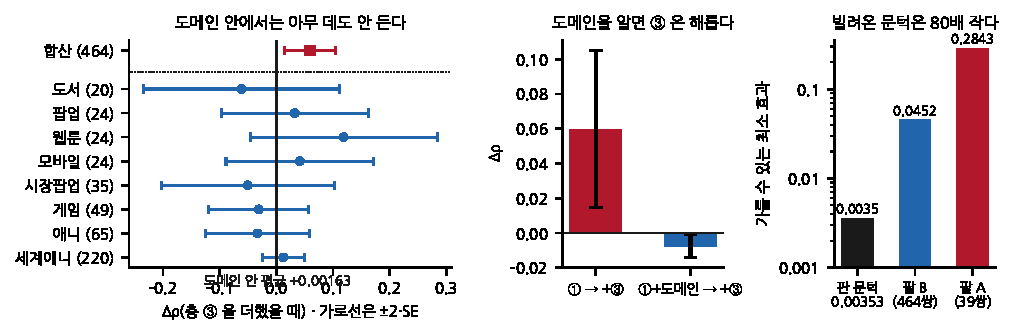
\includegraphics[width=\textwidth]{figs/lay.pdf}
\caption{왼쪽 --- 도메인 안에서는 아홉 중 아무 데도 안 든다(가로선 $\pm2\cdot$SE).
빨간 네모가 합산이다. 가운데 --- 도메인 지시자를 먼저 넣으면 층 ③은 음수 칸으로
내려간다. 오른쪽 --- 빌려온 문턱과 이 자가 실제로 가를 수 있는 최소 효과(로그 축).}
\end{figure*}

\section{물음과 자}

물음은 사용자의 것이다 --- \emph{「state 라는 게 단순히 몇몇 정보가 아니라 그 시기의
관련상황, 혹은 아예 관련없는 상황까지 다 종합되어 나오는 정보들이 반영되어야」}.
그 말을 실험으로 옮기면 \textbf{층을 하나씩 붙이며 예측력이 오르는지}이다.

자는 $\rho_{\mathrm{sao}}$ --- 능형회귀의 교차검증 밖(OOF) 스피어만이다. 겹은
\textbf{개체}로 묶어 같은 개체가 훈련과 시험에 함께 서지 않게 했고, 씨앗 10개의
평균을 값으로 삼는다. 표적은 \textbf{들림} $y=\log_{10}(1+\bar o_{0:14})-
\log_{10}(1+\bar s_{-14:})$ 다. 수준값($\log_{10}(1+\sum o)$)을 안 쓴 이유는
측정 전에 적어 두었다 --- $s$ 의 자기상관이 그것을 $\rho\,0.9334$ 로 이미 맞혀
\textbf{천장에 붙기} 때문이다.

\claimx{판 $\rho$ 의 문턱 $0.00353$ 은 이 자에서 쓸 수 없다. 짝지은 군집
부트스트랩 2{,}000회로 잰 $\mathrm{SE}(\Delta\rho)$ 가 팔 B 에서 $0.0226$,
팔 A 에서 $0.1421$ 이다. 사전등록한 $T=\max(0.00353,\,2\mathrm{SE})$ 는 네 자리
전부에서 $2\mathrm{SE}$ 가 이겼다(12.8배$\sim$80.5배).}{같은 자에서
$2\mathrm{SE}<0.00353$ 이 되면 이 주장은 죽는다 --- 팔 B 를 쌍 $\sim$41{,}000
규모로 키우면 그렇게 된다.}

\section{층 ② --- 자료는 있고 표본이 막는다}

서울 생활인구는 19개월치(2025-01$\sim$2026-07)가 이미 디스크에 있었고 \textbf{쓰는
쌍은 0개}였다. 압축을 풀지 않고 쓸 격자 23개의 줄만 뽑아(468{,}017행) 붙였다.
붙는 쌍은 \textbf{47}, 층 ①·③이 다 있는 것이 \textbf{39}, 서로 다른 격자가 21.

\claimx{층 ②는 이 표본에서 원리상 판정 불능이다. $\Delta\rho=+0.0701$ 이고
$T=0.2843$ · 부트스트랩 95\% 구간이 $[-0.2710,+0.3007]$ 이다. 「안 들었다」가
아니라 \textbf{「못 가른다」}로 적는다.}{쌍을 늘려 $T<|\Delta\rho|$ 가 되면 판정이
생긴다. 지금 좌표가 있는 개체는 133뿐이므로 \textbf{다음 걸음은 생활인구를 더 깊이
읽는 것이 아니라 좌표를 늘리는 것}이다.}

배선은 심은 열로 확인했다 --- ② 자리에 $y$ 에서 만든 열 하나를 넣으면 $\rho$ 가
$-0.0257\to+0.5529$ 로 오른다. \textbf{모형은 열을 받을 수 있다.} 이 검사는 결론의
동어반복이 아니다: 「장이 든다」가 거짓이어도 통과해야 하는 검사이고, 이것이 붉었다면
위 문장을 쓸 자격이 없었다.

\section{층 ③ --- 이득이 어디에 있었나}

합산(464쌍)에서 $\rho$ 는 $0.6400\to0.6998$, $\Delta\rho=+0.0598$ 로 문턱
$0.0452$ 를 넘고 부트스트랩 95\% 구간 $[+0.0180,+0.1064]$ 가 0을 안 문다.
그런데 사전등록한 채택 조건 셋 중 \textbf{라벨 순열 바닥}(상위 5\% $=0.0891$)을
못 넘어 \textbf{채택하지 않았다}. 그리고 더 중요한 것이 도메인별 표에 있었다.

\claimx{층 ③의 이득은 도메인 \emph{사이}의 것이다. 도메인 아홉 중 문턱을 넘는
도메인이 \textbf{0}이고, 쌍 가중 도메인 안 평균 $\Delta\rho$ 가 \textbf{$+0.00163$}
이다(합산 $+0.0598$ 의 2.7\%). 도메인 지시자를 ① 옆에 넣으면 지시자 자신이
$+0.0876$ 을 벌고 그 위에서 ③은 $-0.0075$($T=0.0066$ · 빼는 칸)다.}{어느 한
도메인 안에서 $\Delta\rho>T$ 가 나오면 이 주장은 좁아진다. 표는 그 반대를 보인다 ---
음수 넷 · 양수 넷 · 전부 $\pm2\mathrm{SE}$ 안.}

\textbf{그래서 층 ③은 설계 의도대로 작동하지 않았다.} 의도는 「그 시기 전반이
올랐는지」를 걷어내는 것이었고, 실제로 한 일은 「이 개체가 어느 도메인 크기에
사는지」를 알려 준 것이다. 도메인 이름표는 열 하나로 더 싸게 살 수 있다.

\section{재현성 --- 같은 코드가 다른 수를 냈다}

같은 러너를 15분 간격으로 두 번 돌렸는데 수가 움직였다($\Delta\rho$
$0.0591\to0.0598$ · 도메인 안 평균 $0.00025\to0.00163$). 그 사이 상시 수집
데몬이 배경 곡선의 원천인 위키 일별 파일 열한 개를 다시 썼기 때문이다. 판정 칸은
안 바뀌었지만 \textbf{「같은 코드 · 같은 명령 $\to$ 같은 수」가 거짓}이었다.
데몬을 재우고 정본 주행을 다시 돌렸고, 코드 해시만 박던 자리에 \textbf{입력
해시}를 같이 박았다. 재현 가능성은 코드의 성질이 아니라 \emph{코드와 입력의 짝}의
성질이다.

\section{한계}

생활인구는 서울만이고 2025-01부터라 담론 코퍼스(2012--2023)와 안 겹친다.
「그 격자의 사람이 그 팝업 때문에 왔는가」는 이 자료로 원리상 못 가른다 --- 생활인구는
거주지 기반 추정이라 방문 목적이 없다. 층 ③의 「무관」은 \emph{같은 도메인}으로
좁게 정의했다. 도메인을 가로지르는 배경(진짜 「아예 관련없는 상황」)은 아직 안 쟀다.

\end{document}
